\begin{frame}
    \frametitle{Finite Element Method (FEM)}
    \begin{itemize}
        \item Subdivision of an object into finitely small elements
    \end{itemize}
    \begin{columns}
        \begin{column}{0.4\textwidth}
            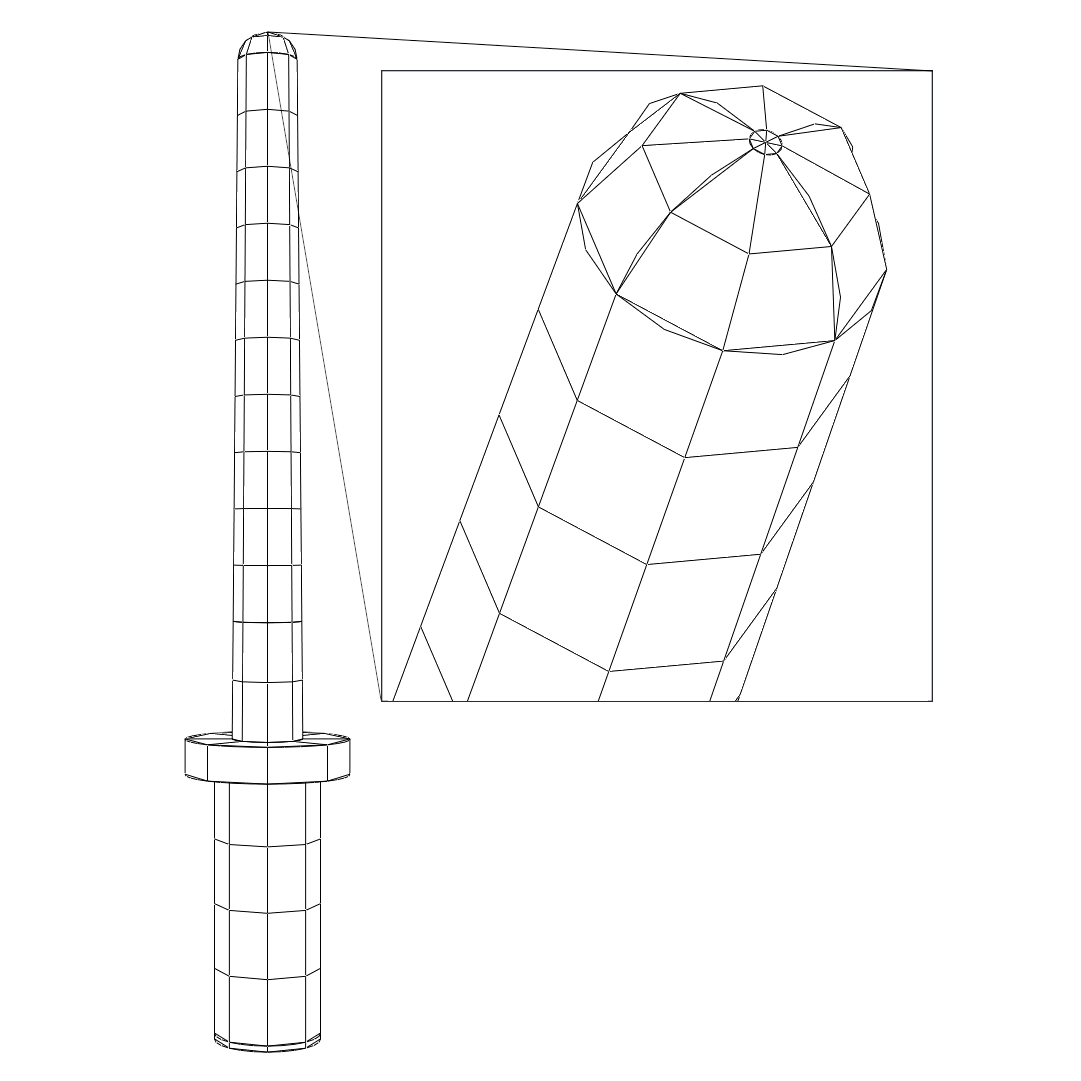
\includegraphics[width=\textwidth]{../figures/0.005-finished.png}
            
        \end{column}
        \begin{column}{0.4\textwidth}
            
\includegraphics[width=0.7\textwidth]{figures/simulia-abaqus.png}
            
\includegraphics[width=0.8\textwidth]{figures/python.png}
        \end{column}
    \end{columns}
\end{frame}

\begin{frame}
    \frametitle{Modelling}
    \begin{itemize}
        \item Key points
        \begin{itemize}
            \alt<1> {
                \item Replicate what will be tested in the lab
            }{}
            \alt<2> {
                \item Simplify and qualify the simplification 
            }{}
        \end{itemize}
    \end{itemize}

    \alt<1>{\vfill
    \begin{center}
        {\tiny \incfig[0.9]{experimental-setup}}
    \end{center}
    }{}
    \alt<2>{
                \begin{center}
                    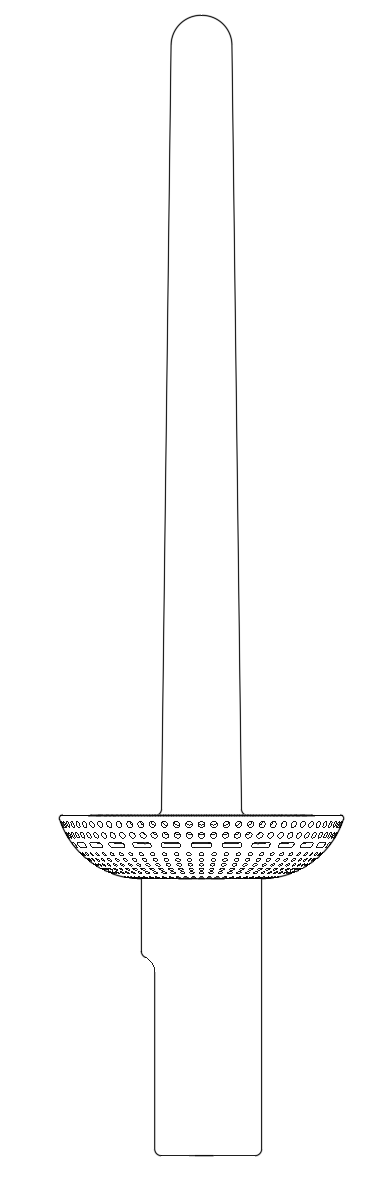
\includegraphics[height = 5cm]{figures/itap-complex.png}
                    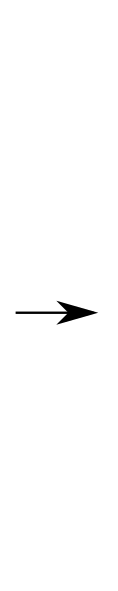
\includegraphics[height = 5cm]{figures/arrow.png}
                    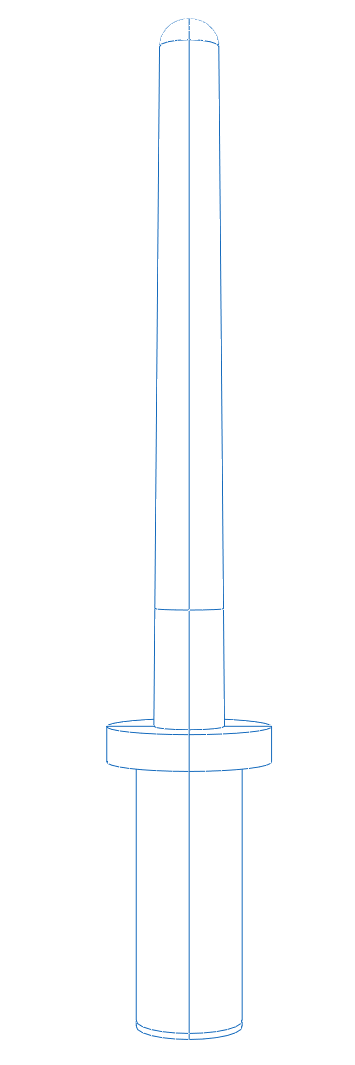
\includegraphics[height = 5cm]{figures/itap-simplified.png}
                \end{center}
    }{}
\end{frame}
